\section{Interactive Plots}

%%%%%%%%%%%%%%%%%%%%%%%
\subsection{\ttfamily rgl \normalfont library} 
%%%%%%%%%%%%%%%%%%%%%%%
\begin{frame}[fragile]
\frametitle{Dynamic visualizations with Package \ttfamily rgl \normalfont}

A way to create 3D interactive images is with the package \ttfamily rgl: \normalfont 

    \begin{columns}
      \column{0.55\textwidth}
\begin{lstlisting}[ basicstyle=\footnotesize ]
library(rgl)
data(quakes)
plot3d(
	x=quakes$long, 
	y=quakes$lat, 
	z=quakes$depth, 
	xlab="Longitude", 
	ylab="Latitude", 
	zlab="Depth"
	)
\end{lstlisting}
%g <- expand.grid(x = 1:10, y = 5:15)
%g$z<-g$x^2
%wireframe(g$z~g$x*g$y, scales = list(arrows = FALSE), drape = TRUE, colorkey = TRUE)

     \column{0.45\textwidth}
       \begin{center}
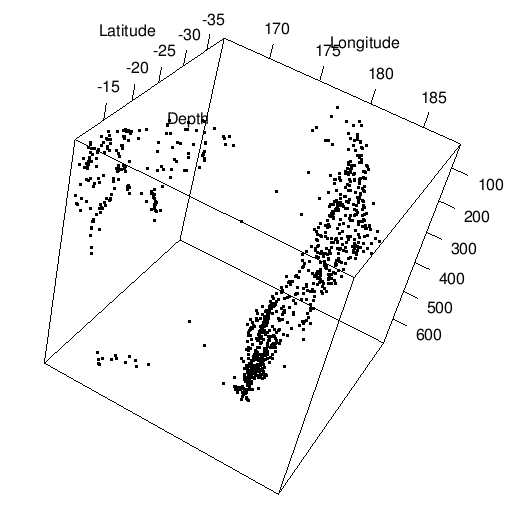
\includegraphics[width = 55mm]{images/Fiji_RGL}
\end{center}
\end{columns}
\end{frame}

%------------------------------------
\subsection{\ttfamily ??? \normalfont library} 
%------------------------------------
\begin{frame}[fragile]
	\frametitleDynamic Visualizations with Package \ttfamily ??? \normalfont}
\end{frame}

%------------------------------------
\subsection{\ttfamily shiny \normalfont library} 
\begin{frame}[fragile]
	\frametitle{Interactive visualizations with Package \ttfamily shiny \normalfont}
\end{frame}
%------------------------------------

% ------------------------------------------------------------
% ------------------------------------------------------------
\subsection{Exercise IV}
\begin{frame}
	\frametitle{Exercise IV}
	Use the \ttfamily rgl \normalfont library to create a 3D plot of the \ttfamily ozone \normalfont data set \footnote{\ttfamily http://www.ats.ucla.edu/stat/R/faq/ozone.csv\normalfont}.
\end{frame}